\subsection{Results}

It is challenging to get the network to learn stable and well. Here I present the learning process for variouse sizes of the replay buffer and look at the effect of infrequent weight updating. We take a look at what these changes mean for learning stability. The paramaters in \autoref{tab:shared_params} are shared between all results.

\begin{table}[ht]
  \centering
  \fontfamily{ppl}\selectfont
  \begin{tabular}{ll}
    \toprule
    Paramater & Value \\
    \midrule
    discount factor $\gamma$ & $0.95$ \\
    replay sample size & $32$ \\
    maximum steps & $200$ \\
    training sessions & $1000$ \\
    learning rate & $0.001$ \\
    epsilon start & $5$ \\
    epsilon decay & $5^{-5}$ \\
    \bottomrule
  \end{tabular}
  \caption{The paramaters and theire values shared between all mountain car results.}
  \label{tab:shared_params}
\end{table}

The default size of the replay buffer is $20000$ timesteps or events. We start by looking at the learning behaviour of the agent with this size of buffer. Because reinforced learning can be unreproducible, especially when combined with the unreproducibility of neural networks we train 4 times. The results are in \autoref{fig:mcar_20k_a} and \autoref{fig:mcar_20k_b}.

\begin{figure}
    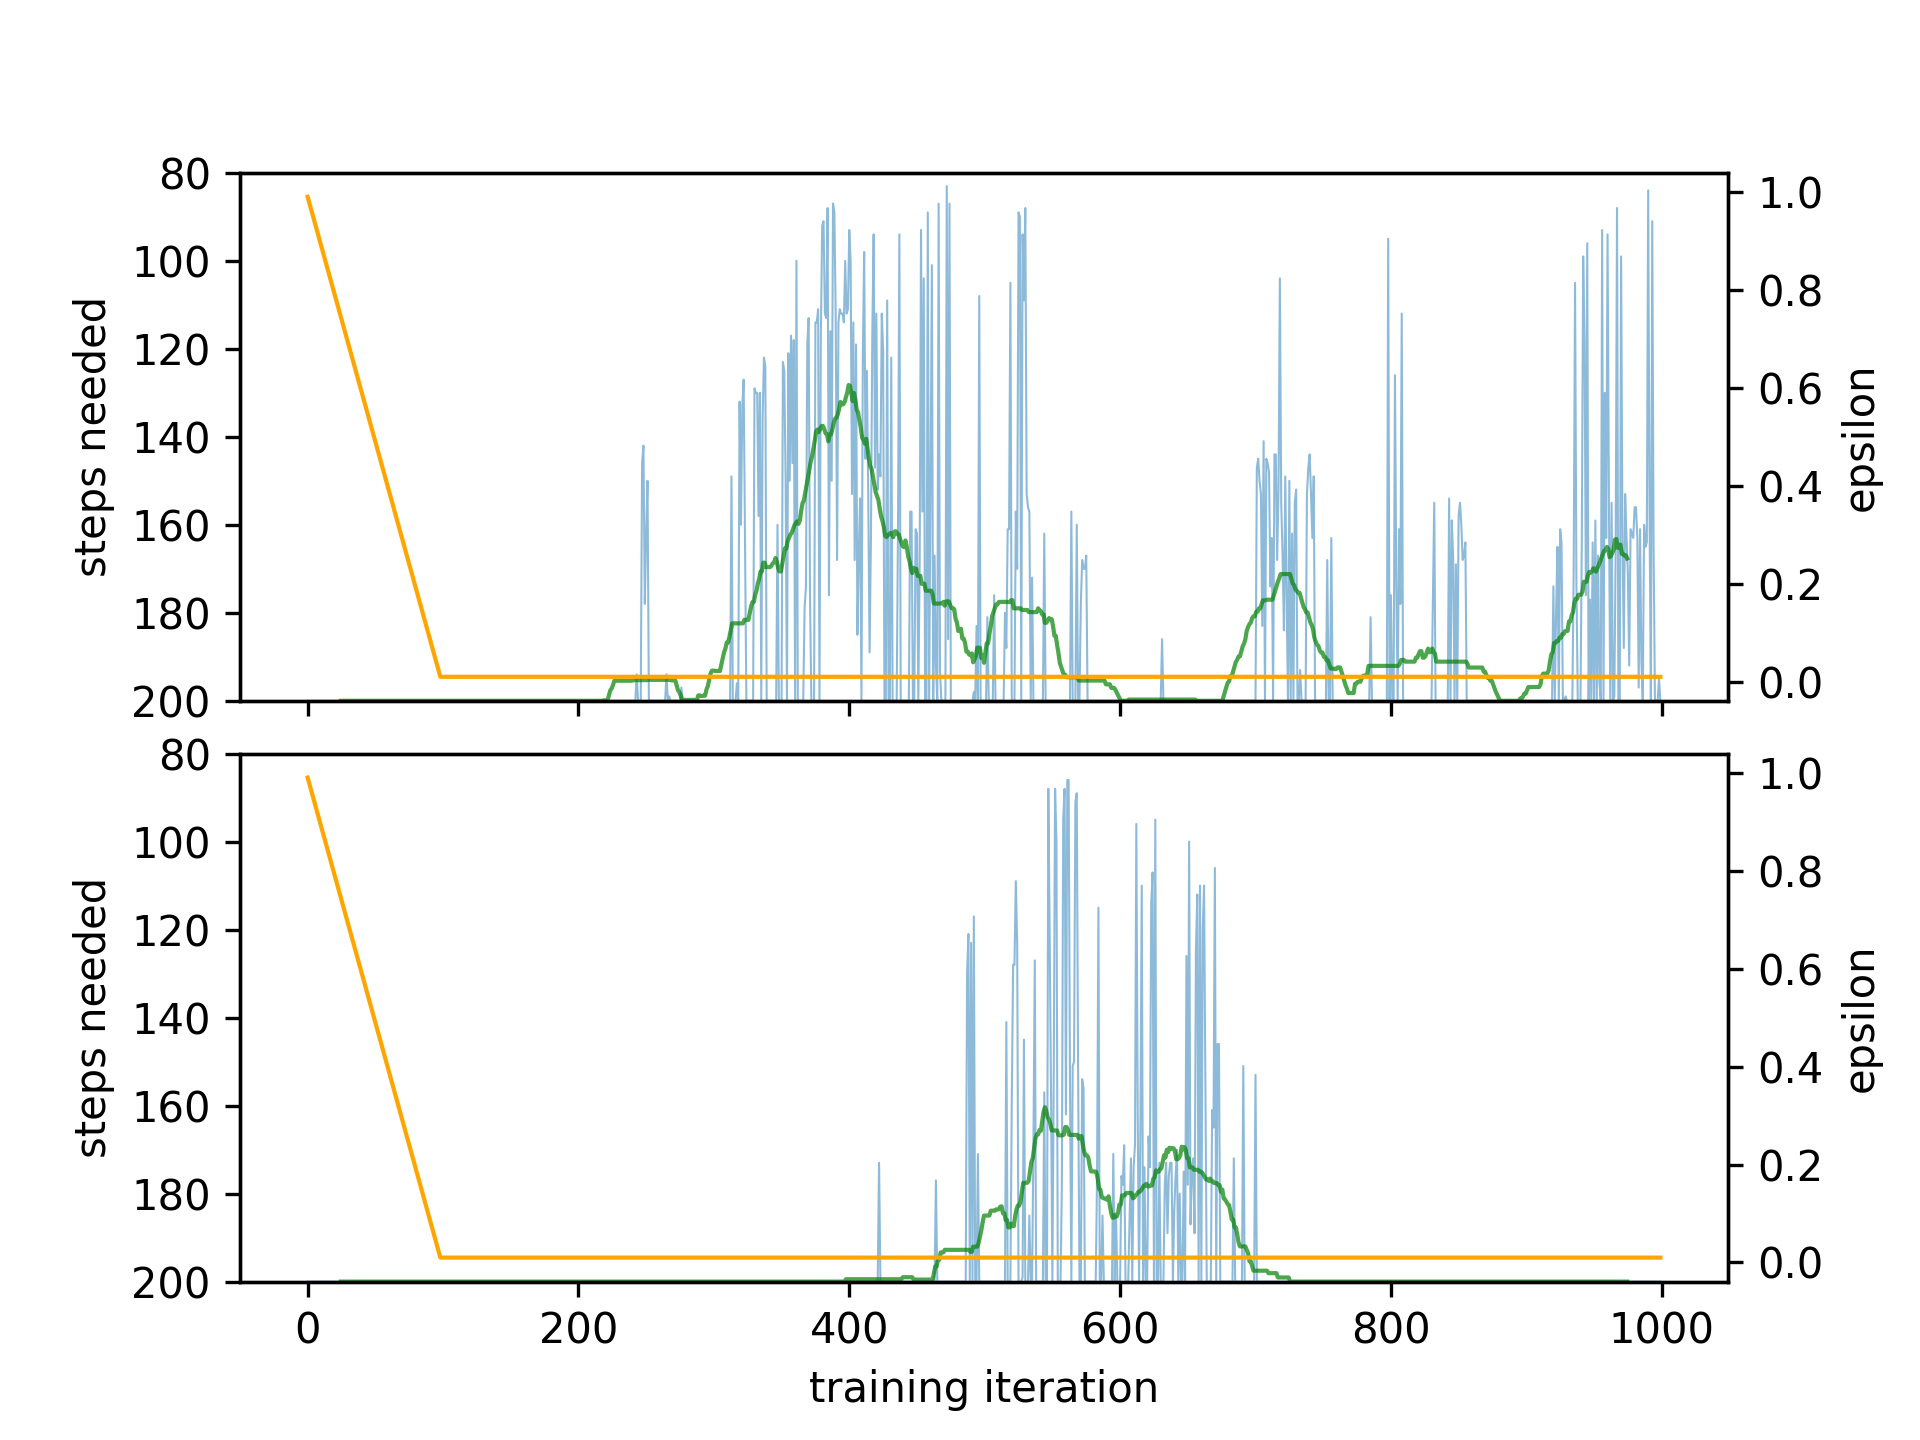
\includegraphics{mcar_20000_a}
    \caption{Two seperate runs of training the mountain car agent with a replay buffer which remembers the last $20000$ timesteps. On the y-axis the number of steps needed to finish, 200 means the algorithm failed to reach the goal in time. On the x-axis the session number. Note how both attempts do not lead to convergence within 1000 steps}
    \label{fig:mcar_20k_a}
\end{figure}

\begin{figure}
    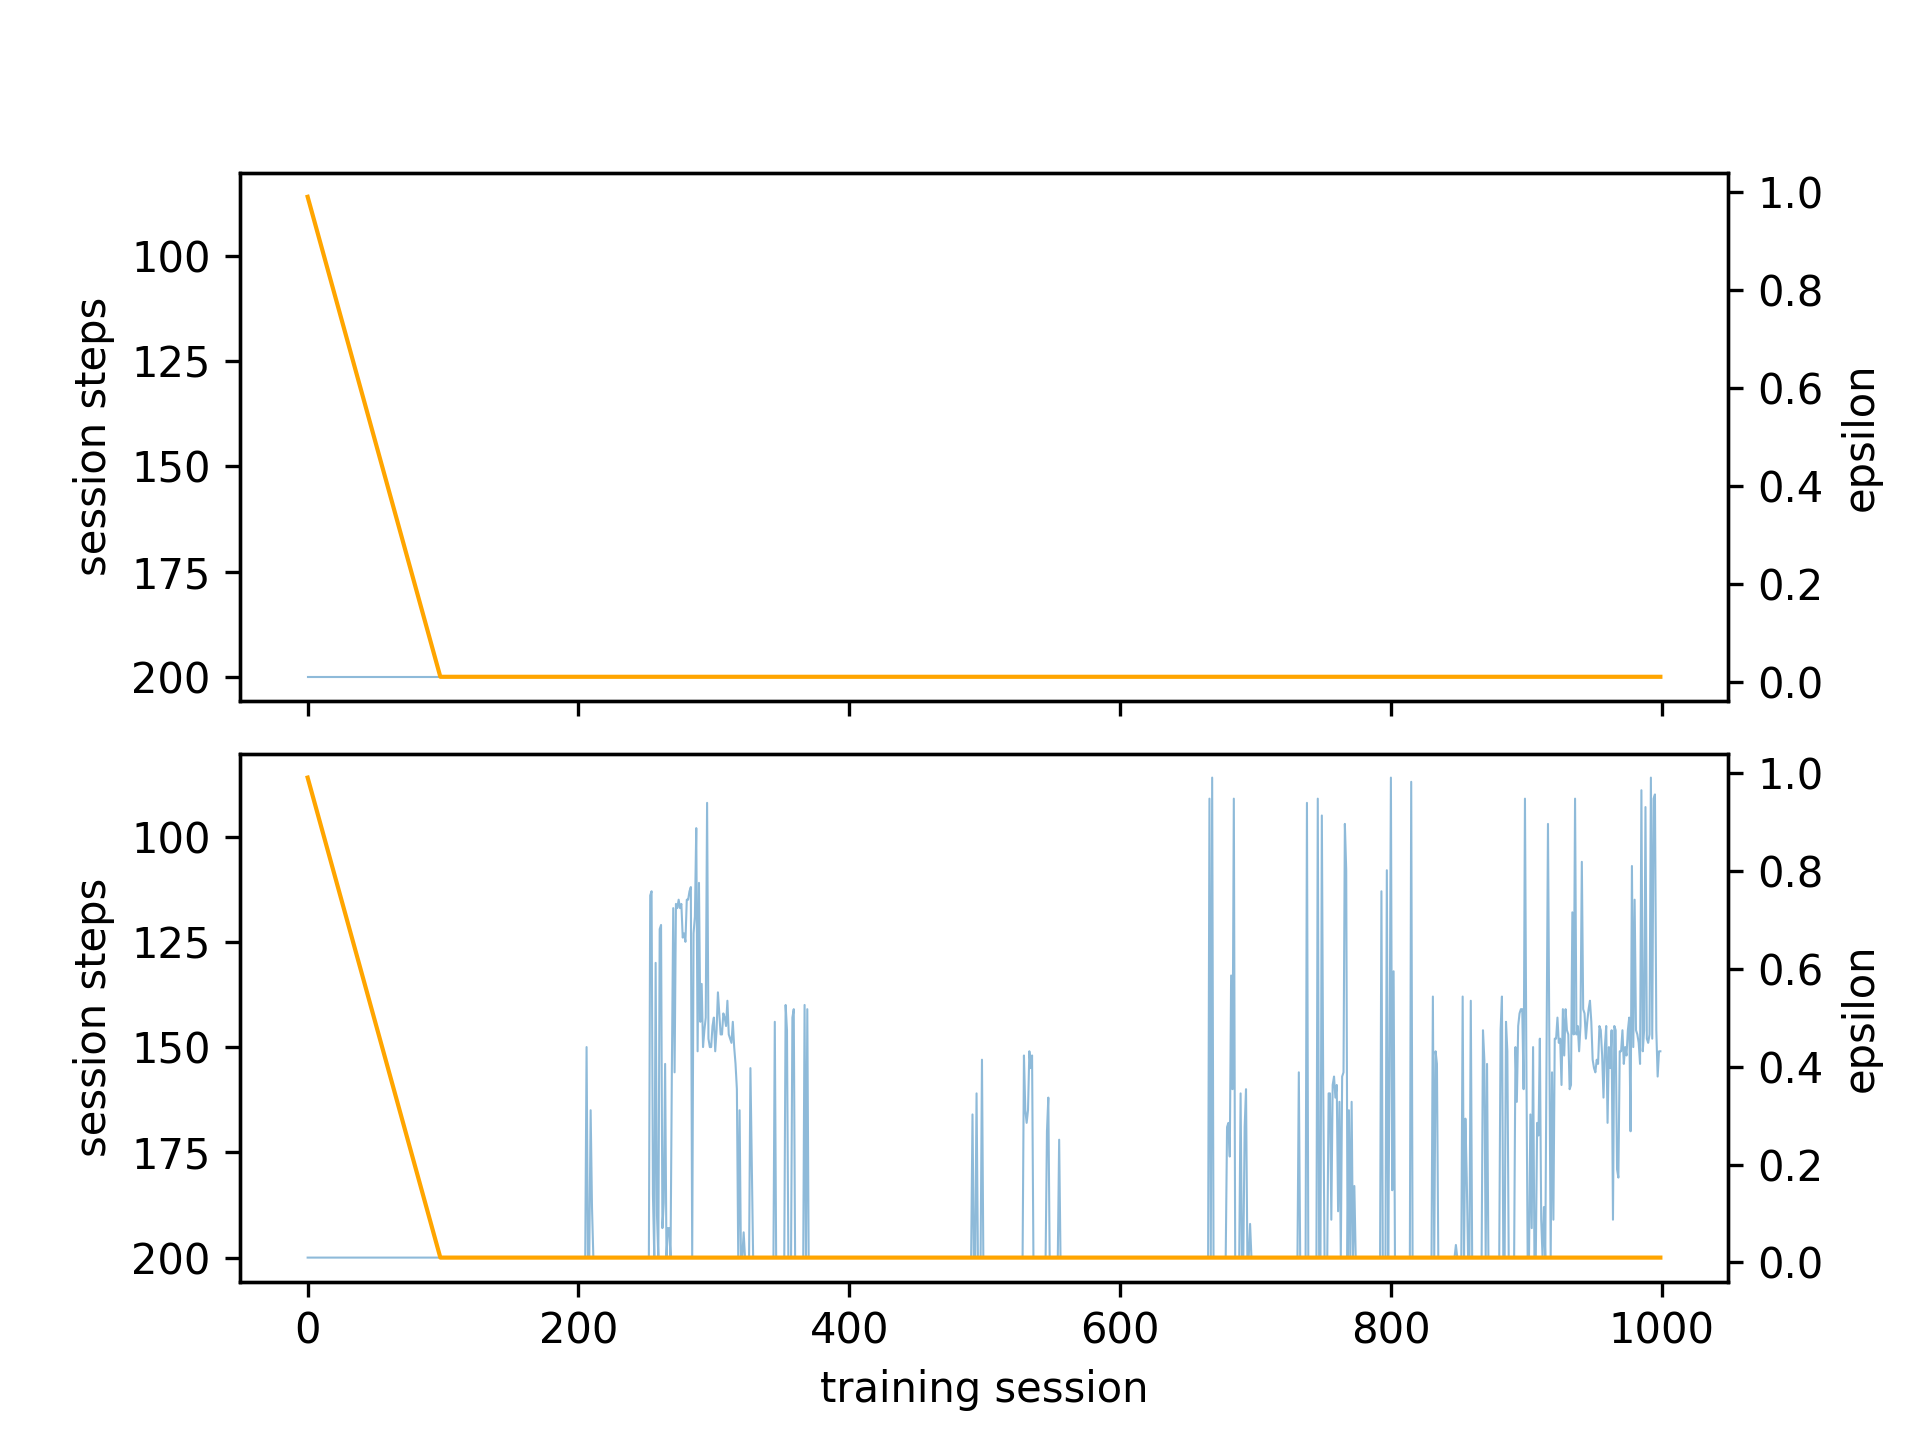
\includegraphics{mcar_20000_b}
    \caption{Two seperate runs of training the mountain car agent with a replay buffer which remembers the last $20000$ timesteps. On the y-axis the number of steps needed to finish, 200 means the algorithm failed to reach the goal in time. On the x-axis the session number. Note that top run never succeeded in the task while the bottom started to converge at around session 900.}
    \label{fig:mcar_20k_b}
\end{figure}

We see that the agent remains unrelaible in most cases, sometimes it never even starts getting results (see \autoref{fig:mcar_20k_b}). Other times it starts producing good results before failing at the task again 200 sessions later as we see in the bottem screen of  \autoref{fig:mcar_20k_a}

Now we look at the learning stability of the agent if we decrease the buffer size, we expect the stability to decrease as the deadly triad becomes a larger problem and we start biting in our own tail again. In \autoref{fig:mcar_10k_a} and \autoref{fig:mcar_10k_b} we see the learning behaviour of the agens with a replay buffer of $10 000$ timesteps.

\begin{figure}
    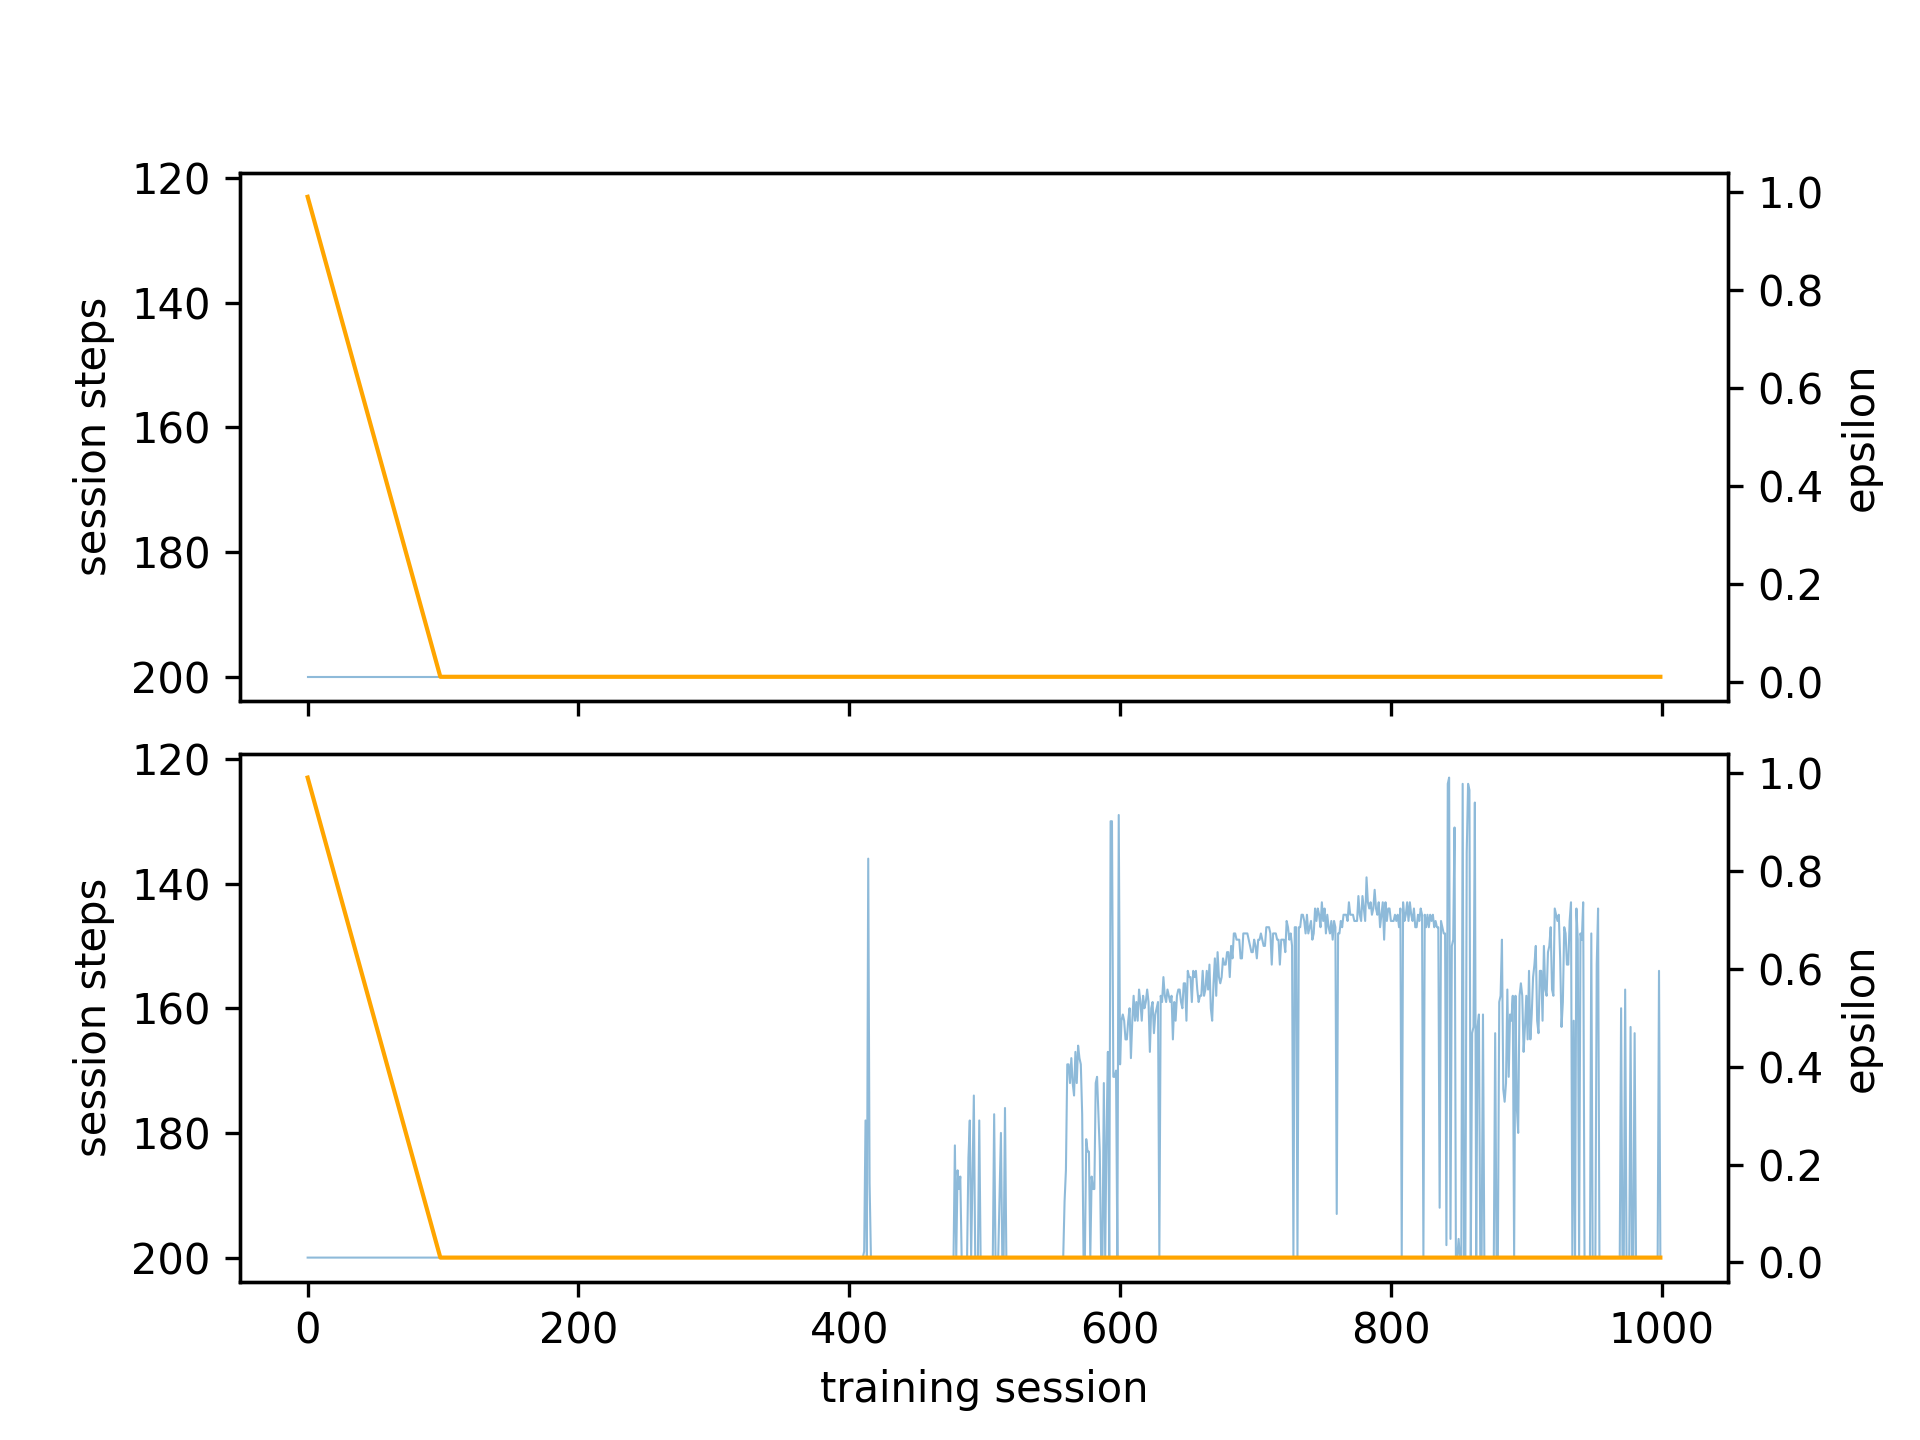
\includegraphics{mcar_10000_a}
    \caption{Two seperate runs of training the mountain car agent with a replay buffer which remembers the last $10000$ timesteps. On the y-axis the number of steps needed to finish, 200 means the algorithm failed to reach the goal in time. On the x-axis the session number. TODO}
    \label{fig:mcar_10k_a}
\end{figure}

\begin{figure}
    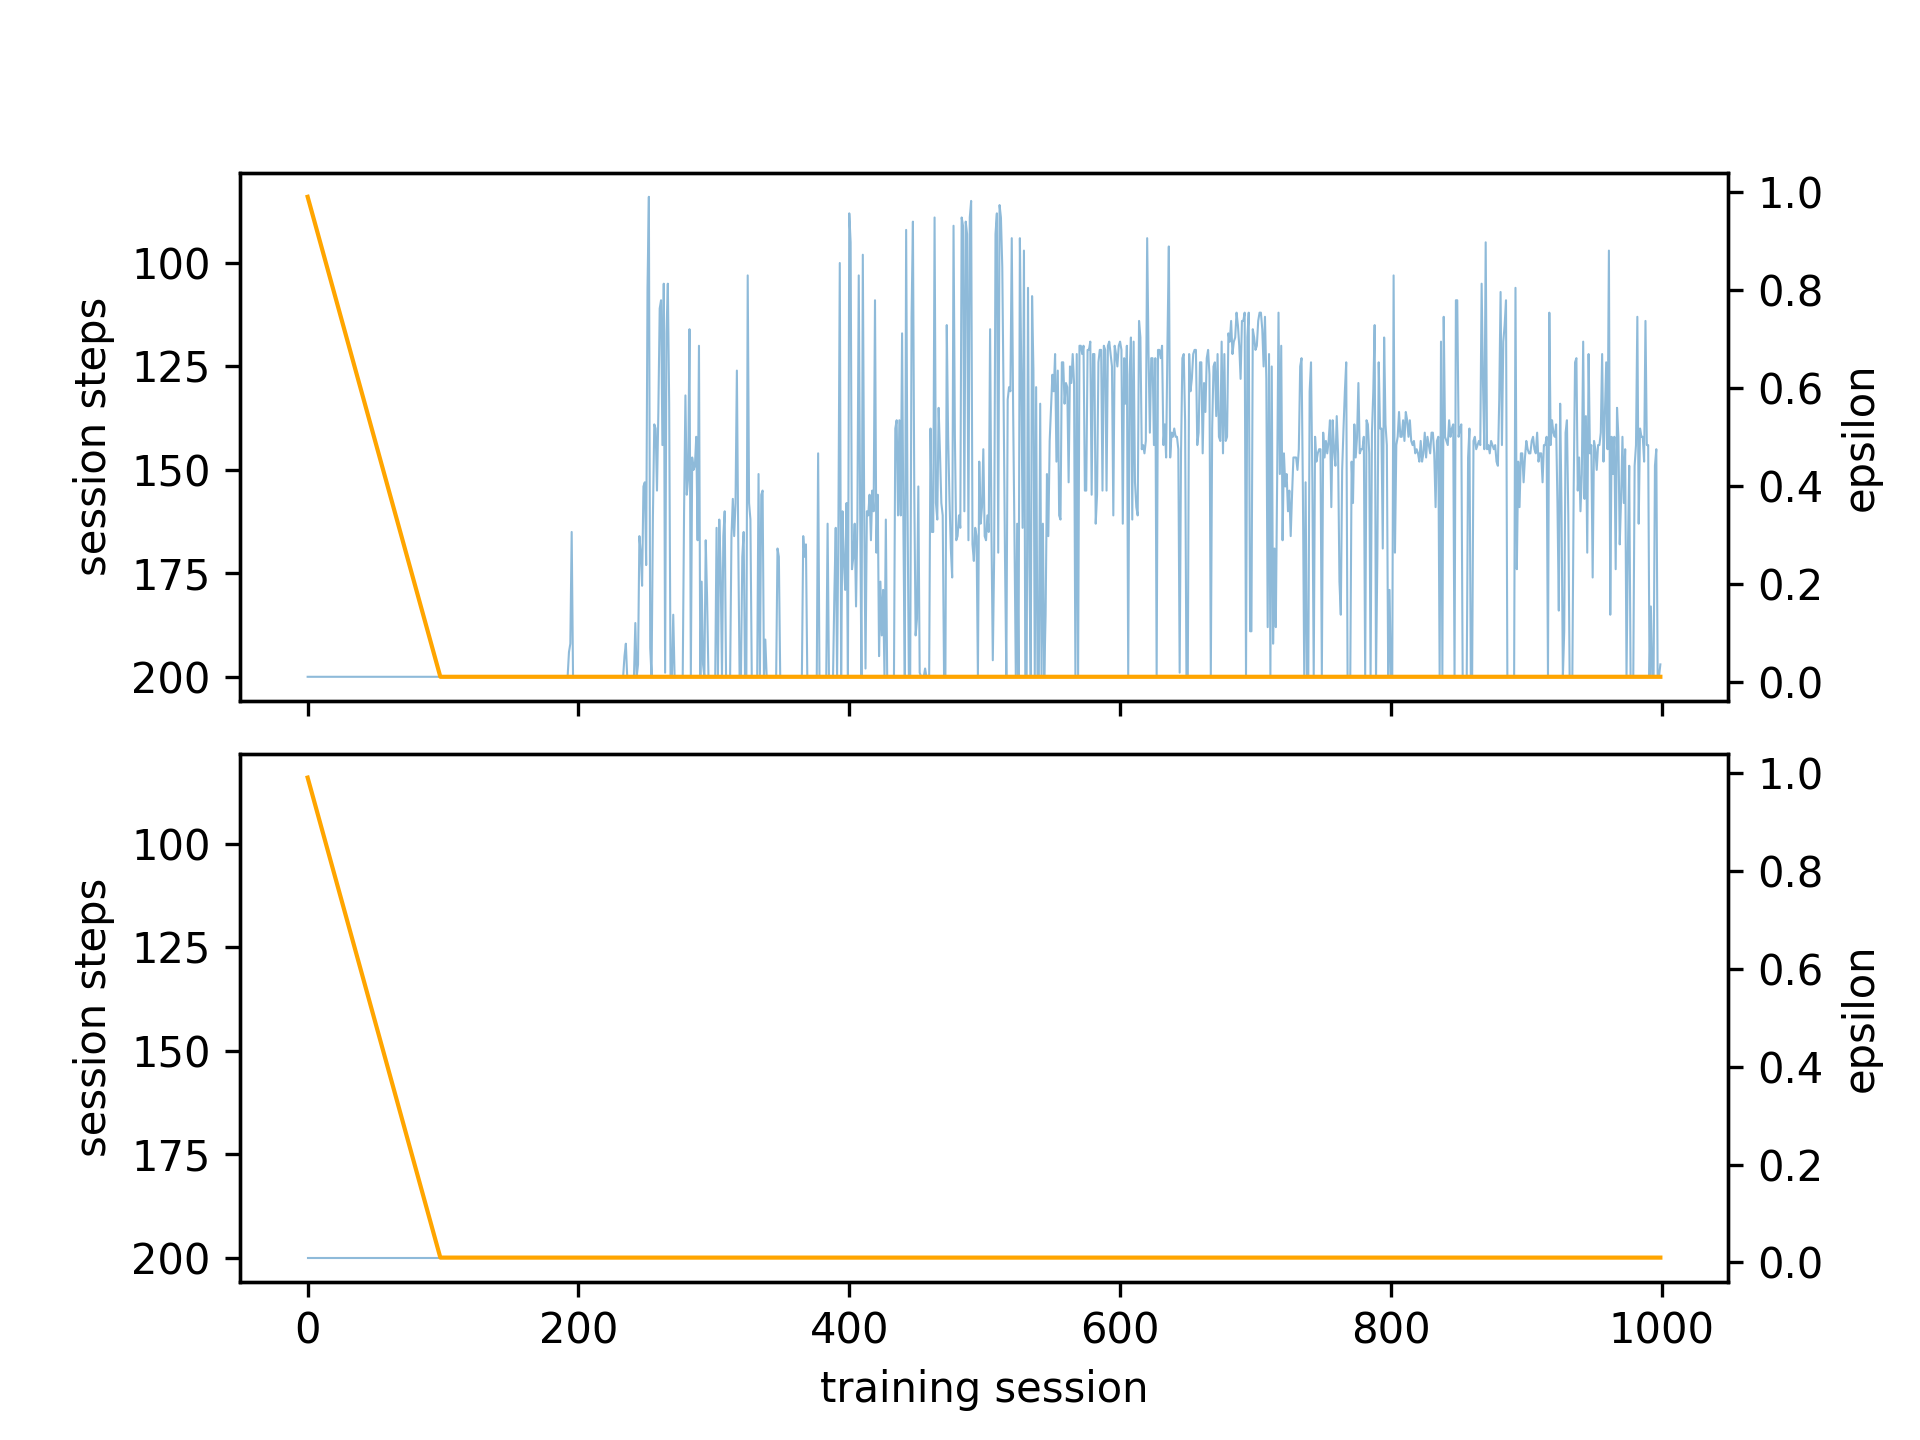
\includegraphics{mcar_10000_b}
    \caption{Two seperate runs of training the mountain car agent with a replay buffer which remembers the last $10000$ timesteps. On the y-axis the number of steps needed to finish, 200 means the algorithm failed to reach the goal in time. On the x-axis the session number. TODO.}
    \label{fig:mcar_10k_b}
\end{figure}